\documentclass{replab}
\usepackage{lipsum}
\usepackage[shortlabels]{enumitem}
\usepackage{amsmath}
\usepackage{physics}
\usepackage{bm}

% --- Información del documento ---
\title{Física - Cinemática}
\author{Diego Alejandro Heredia Franco}

% Nota: Si se desea incluir más de un autor en el documento, el archivo replab.cls, en la sección "Página de título de documento", contiene líneas de código comentadas pensadas para introducir los datos desde 1 hasta 4 autores. Sin embargo, debe escogerse solo una de las cuatro secciones de código y comentar las demás para mantener la consistencia del documento.

\date{21/22 de mayo de 2025}
\subtitle={Taller Calificable 1}
\email={\href{mailto:dherediaf@unal.edu.co}{\color{principaluno}\texttt{dherediaf@unal.edu.co}}}
\subject={Taller Fundamentos de Mecánica}

\setlength{\columnsep}{14pt}

% --- Archivo de bibliografía ---
\addbibresource{repbib.bib}

% --- Inicio del documento ---
\begin{document}
\setlength{\parindent}{0pt}
	
	\pagestyle{fancy}
	\unspacedoperators
	
% --- Título ---
	{\begin{tcolorbox}[colframe=green!50!black, colback=green!20!white, arc=8pt]
		\begin{center}
			\maketitle
			%\rule{\textwidth}{0.2pt}
			%\medskip

			%\noindent\textit{Palabras Clave:} medidas directas e indirectas, análisis estadístico, incertidumbre, calibrador Vernier, balanza.
		\end{center}
	\end{tcolorbox}}
	\selectlanguage{spanish}

	Los ejercicios que aquí se presentan, han sido tomados de \cite{lanaturaleza}, \cite{serway}, \cite{londono} y \cite{sears} en los capítulos relacionados con cinemática y movimiento rotacional.\\

	\textbf{\textit{Parámetros de Entrega:}} Se espera que trabajen en grupos de entre 2 a 3 personas. El taller debe ser entregado en formato digital (PDF), uno por cada miembro del grupo, y subido a una carpeta compartida en Google Drive. Cada grupo debe crear su propia carpeta y compartir el link con el profesor.\\

{\begin{tcolorbox}[colframe=red!50!black, colback=red!5!white, arc=8pt]
	\textbf{\textcolor{red!50!black}{Sugerencia:}} En el libro \textit{Física Universitaria Vol.1} (Zemansky) \cite{sears}, se presenta al final de cada sección un \textit{\textbf{resumen de los conceptos más importantes}}, así como un pequeño manuscrito con una \textit{\textbf{estrategia para resolver problemas}}. Se recomienda al estudiante leer este instructivo para que pueda resolver los ejercicios de forma más organizada y eficiente.
\end{tcolorbox}}

% --- Cuerpo del reporte ---
\section{Ejercicios Introductorios}

\subsection{Notación Científica y Redondeo}
Redondee las siguientes cantidades hasta el numero indicado de cifras significativas (cs): \textbf{(a)} $132.505g$ (4cs), \textbf{(b)} $13.452lb$ (2cs), \textbf{(c)} $345onzas$ (2cs), \textbf{(d)} $7.4855g$ (3cs), \textbf{(e)} $11.698lb$ (1cs), \textbf{(f)} $12.05$ (3cs).

\subsection{Mínima Área Superficial}
Demuestre que un cilindro recto con determinado volumen $V$ tiene un área superficial mínima cuando su altura $h$ es igual a su diámetro $d$. El kilogramos patrón se fabricó según este criterio para reducir al mínimo los errores debidos a la contaminación o corrosión de su superficie. 

\section{Ejercicios Vectores}

\subsection{Coordenadas Polares}
Sean $(r,\theta)$ las coordenadas polares del punto $(x,y)$. Determine las coordenadas polares para los puntos \textbf{a)} $(-x,y)$, \textbf{b)} $(-2x,-2y)$, y \textbf{c)} $(3x,-3y)$.

\subsection{Magnitud y Dirección}
Dos vectores $\vec{A}$ y $\vec{B}$ tienen magnitudes exactamente iguales, $|\vec{A}| = |\vec{B}|$. Para que la magnitud de $\vec{A} + \vec{B}$ sea 100 veces mayor que la magnitud de $\vec{A} - \vec{B}$, ¿Cuál debe ser el ángulo entre ellos?. (R: $1.15^\circ$)

\section{Ejercicios Cinemática 1D}

\subsection{Canica sobre una Pista}
Una niña rueda una canica sobre una pista con dobleces que mide $100cm$ de largo, como se muestra en la (Fig. \ref{fig:pista2}). Use x para representar la posición de la canica a lo largo de la pista. En las secciones horizontales de $x=0cm$ a $x=20cm$ y de $x=40cm$ a $x=60cm$, la canica se mueve a una rapidez constante. En las secciones de pendiente, la rapidez de la canica cambia de manera uniforme. En los lugares donde la pendiente cambia, la canica permanece en la pista y no experimenta cambios súbitos de rapidez. La niña da a la canica cierta rapidez inicial en $x=0cm$ y $t=0s$ y luego la observa rodar a $x=90cm$ donde regresa, y eventualmente regresa a $x=0cm$ con la misma rapidez inicial con la que al inicio la niña la liberó. Prepare graficas de $x$ en función de $t$, de $v_x$ en función de $t$ y de $a_x$ en función de $t$. 
	
\begin{figure}[htbp]
	\centering
	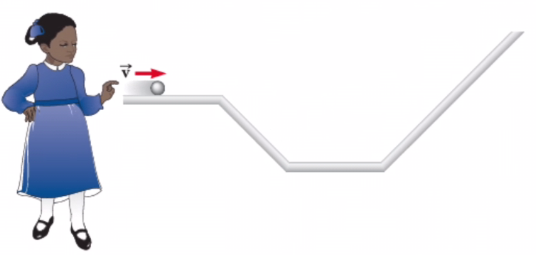
\includegraphics[width=.4\columnwidth]{imagenes/pista2.png}
	\caption{Dibujo esquemático de la pista para la canica.}
	\label{fig:pista2}
\end{figure}

\subsection{Distancia Relativa}
	Un globo \textit{asciende} con velocidad constante de $10m/s$. En cierto momento su tripulante deja caer una piedra sin comunicarle ningún impulso. Halle la distancia entre el globo y la piedra en función del tiempo. Resuelva el ejercicio \textbf{a)} desde la perspectiva de un observador en el globo y \textbf{b)} desde la perspectiva de un observador en la tierra. Evalúela a los $5s$, en ambos casos el resultado debe ser el mismo.\\ 

	\textbf{Nota:} Defina bien su marco de referencia y piense cual es la velocidad inicial de la piedra en cada uno.

\section{Ejercicios Cinemática 2D}

\subsection{Movimiento de un Proyectil}
Un proyectil se lanza desde un risco de altura $h$ y a un ángulo $\theta$ respecto al horizonte. Si la rapidez inicial del proyectil es $v$, calcule \textbf{a)} la altura máxima que alcanza el proyectil y el tiempo en llegar a la altura máxima, \textbf{b)} el tiempo total de vuelo, y \textbf{c)} el alcance del proyectil (distancia horizontal a la que cae el proyectil en el suelo).

\subsection{Intercepción}
Un objeto es lanzando (bajo acción del campo gravitacional) con una velocidad inicial $v_1$ que forma un ángulo $\theta$ con la horizontal. En ese mismo instante otro objeto es lanzado verticalmente con velocidad inicial $v_2$, separado una distancia $D$ del primer proyectil. Si los dos proyectiles chocan en el aire y las magnitudes de las velocidades están relacionadas por $v_1 = \sqrt{2}v_2$, \textquestiondown cuál es el valor de $\theta$ y en qué tiempo ocurre la colisión? \textquestiondown Qué relación debe tener $D$ y $v_1$, para que en efecto la colisión ocurra? Véase la Fig. \ref{fig:interception}.

\begin{figure}[htbp]
	\centering
	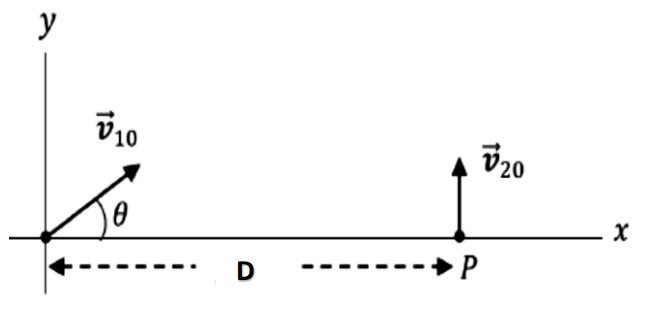
\includegraphics[width=.4\columnwidth]{imagenes/interception.png}
	\caption{Colisión de dos partículas en el aire.}
	\label{fig:interception}
\end{figure}

\subsection{Colisión de un Proyectil}
Se lanza desde el piso un proyectil con velocidad de $15m/s$ y un ángulo de $\psi$ con la horizontal.

\begin{enumerate}[a)]
	\item Calcule el máximo alcance horizontal (R/ $22.96m$).
	\item Si hay una pared vertical a $18m$ del punto de lanzamiento, ¿con qué ángulo debe lanzarse la bala para golpear la pared lo mas alto posible y cuánto vale esa altura? En el momento en que la bola golpea la pared, ¿está subiendo o bajando? (R/ $51.90^{\circ}; 4.42m$)
	\item Si además de la pared vertical hay un techo horizontal a $4.5m$ sobre el piso, ¿Cuál es ahora el punto más alto en el que puede golpearse la pared vertical con la bala y con qué ángulo debe lanzarse? (R/ $38.76^{\circ}; 2.85m$)
\end{enumerate}

\section{Ejercicios Movimiento Rotacional}

\subsection{\textit{FPS} vs Movimiento Continuo}

	En películas cinematográficas y de televisión es común observar los neumáticos de los vehículos girando en sentido contrario a lo esperado. El efecto se debe a que el registro cinematográfico no es continuo y permanente, sino que se realiza típicamente a razón de $24$ imágenes por segundo ($24$ FPS).

	\begin{enumerate}[a)]
		\item ¿Cúal es la rapidez aparente de un automóvil cuyos neumáticos de $60cm$ de diámetro parecen girar en retroceso a razón de $\pi/3$ radianes por segundo? (R: $-1.13km/h$)
		\item ¿Cúal puede ser la rapidez real del automóvil? Haga un esquema que ilustre la situación? (R: $143\pi/3 rad/s$)
		\item ¿Es posible que el efecto estroboscópico haga que su respuesta no sea unívoca, es decir, que existan otras velocidades que también cumplan con el enunciado del problema? Haga un comentario al respecto.
		\item Si el automóvil se mueve a $97.2km/h$, ¿A qué velocidad angular aparente giran los neumáticos? (R: $-0.23rad/s$)
	\end{enumerate}

\subsection{El Carrusel}
\textbf{a)} ¿Cuál es el periodo y velocidad de una persona en un carrusel, si la persona experimenta una aceleración de magnitud $0.80m/s^2$ cuando esta a $4.0m$ del eje de rotación? \textbf{b)} ¿Cuál es la magnitud de la aceleración y la velocidad si ahora la persona se ubica a $2.0m$ del centro del carrusel? Asuma que el carrusel se mantiene rotando con el mismo periodo.

\subsection{Vector Aceleración}
Un automóvil de carreras parte del reposo en una pista circular; aumenta su rapidez a una cantidad constante $a$, conforme da una vuelta a la pista. Encuentre el ángulo que forma la aceleración total del automóvil, con el radio que conecta el centro de la pista y el auto, en el momento en que el automóvil completa el círculo.

\subsection{Centrifuga de Laboratorio}
\textbf{Aplicación Biológica} 

La sangre humana contiene plasma, plaquetas y glóbulos rojos. Para separar el plasma de los otros componentes, se utiliza la centrifugación. Una centrifugación efectiva requiere someter la sangre a una aceleración de $2000g$ o más. En este caso, se asume que la sangre está contenida en tubos de ensayo de $15cm$ de largo y completamente llenos de sangre. Estos tubos giran en la centrífuga inclinada a un ángulo de $45^\circ$ por encima de la horizontal (Fig. \ref{fig:centrifuga}).

% Para hacer un espacio dentro de una ecuacion se utiliza \,

\begin{enumerate}
	\item[a)] ¿Cuál es la distancia de una muestra de sangre al eje de rotación de una centrífuga que gira a $3500\,\text{rpm}$, si tiene una aceleración de $2000g$?

	\item[b)] Si la sangre en el centro de los tubos gira alrededor del eje de rotación a la distancia calculada en el apartado (a), calcula las aceleraciones que experimenta la sangre en cada extremo del tubo de ensayo. Expresa todas las aceleraciones como múltiplos de $g$.
\end{enumerate}


\begin{figure}[htbp]
	\centering
	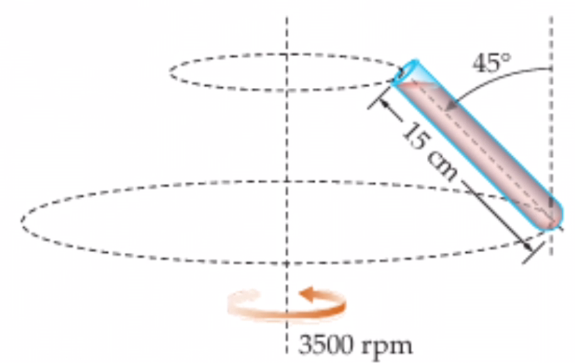
\includegraphics[width=.4\columnwidth]{imagenes/centrifuga.png}
	\caption{Dibujo esquemático de la centrifuga de laboratorio.}
	\label{fig:centrifuga}
\end{figure}



\printbibliography[heading=bibintoc]
	
\end{document}